\documentclass{article}
\usepackage{graphicx}
\usepackage{amssymb}
\usepackage[utf8]{inputenc}
\usepackage{geometry}
\usepackage{hyperref} %Este paquete es para los URL o Links.
\geometry{left=1in, right=1in, top=1in, bottom=1in}
\title{\bfseries Collection} 
%\vspace{-1cm}; recordar este comando para dismuir la separación
\author{Alejandra Marulanda Gallego}
\begin{document}
\maketitle
\section{Tesis Valeria (Modelo molecular exacto para los estados S de los átomos de dos electrones. Aplicación al estado basal del He y de su serie isoelectrónica)}
Se introdujo una factorización exacta y única de la función propia
en términos de una amplitud marginal. Está depende funcionalmente
de la distancia interelectrónica (r12) y de una amplitud condicional,
la cual a su vez depende funcionalmente de las distancias electrón-núcleo
r1,r2 y paramétricamente de r12. Luego, se aplicó el principio variacional 
deduciendo así las ecuaciones de valor propio para las dos amplitudes.\newline
\textbf{La ecuación marginal} incluye un hamiltoniano efectivo, el cual
contiene una curva de energía potencial no adiabática que toma en cuenta 
todas las correlaciones entre las partículas de manera promediada, cuyo 
valor propio único es la energía interna. Por otro lado, en cada punto r12 
tal curva es, a su vez, el valor propio único en \textbf{la ecuación condicional}.\newline
\textbf{En conclusión}, empleando el estado basal del He y de su serie 
isoelectrónica como prototipo, se demostro que dicha curva proporciona una
interpretación de la estructura del átomo análoga a la de una molécula 
diatómica.\newline
La ecuación de Schrödinger para los sistemas atomicos conformados 
por más de un electrón no tiene solución exacta debido a las repulsiones
interelectrónicas.   
\section*{Conceptos}
\subsection*{Tesis Valeria}
\begin{itemize}
    \item \textbf{Factorización exacta:} 
    \item \textbf{Función propia:}
    \item \textbf{Amplitud marginal:}
    \item \textbf{Distancia interelectrónica:}
    \item \textbf{Amplitud condicional:}
    \item \textbf{Dependencia funcional:}
    \item \textbf{Dependencia parametrica:}
    \item \textbf{Principio variacional:}
    \item \textbf{Ecuación de valor propio:}
    \item \textbf{Ecuación marginal:}
    \item \textbf{Hamiltoniano efectivo:}
    \item \textbf{Curva de energía potencial:}
    \item \textbf{No adiabática:}
    \item \textbf{Correlaciones:}
    \item \textbf{Valor propio:}
    \item \textbf{Ecuación condicional:}
\end{itemize}
\section{Formalismo}
Coordenadas de Hylleraas:
Hylleraas mostró que la función de onda electrónica para
cualquier estado S de un átomo de dos electrones, considerando
el centro de masa el núcleo, se puede factorizar en una parte 
angular y otra interna, donde la última se puede expresar en 
términos de r1, r2 y r12. 

\begin{figure}[htb]
    \centering
    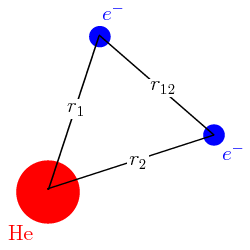
\includegraphics[width=5cm, height=5cm, scale=0.5]{modelo_de_atomo_de_helio.PNG}
    \caption{Modelo de atomo de helio.}
\end{figure}

Estas coordenadas determinan la forma y el tamaño del triángulo
electrón-núcleo-electrón y son independientes entre sí, excepto 
que deben satisfacer la desigualdad triagular:\newline

\begin{center}
\mid r12-r2\mid \leqslant r1 \leqslant r12+r2 
\end{center} \newline

Por otro lado, la función angular determina la orientación de 
dicho triángulo en el espacio. Para nuestros propósitos, no se 
necesita especificar esta función, debido a que los estados S 
tienen simetría esférica. Por lo tanto, la ecuación de Schrödinger
interna,\newline

\begin{center}

\end{center}

\end{document}